\begin{figure}
    \centering
    \begin{subfigure}[c]{0.48\linewidth}
        \centering
        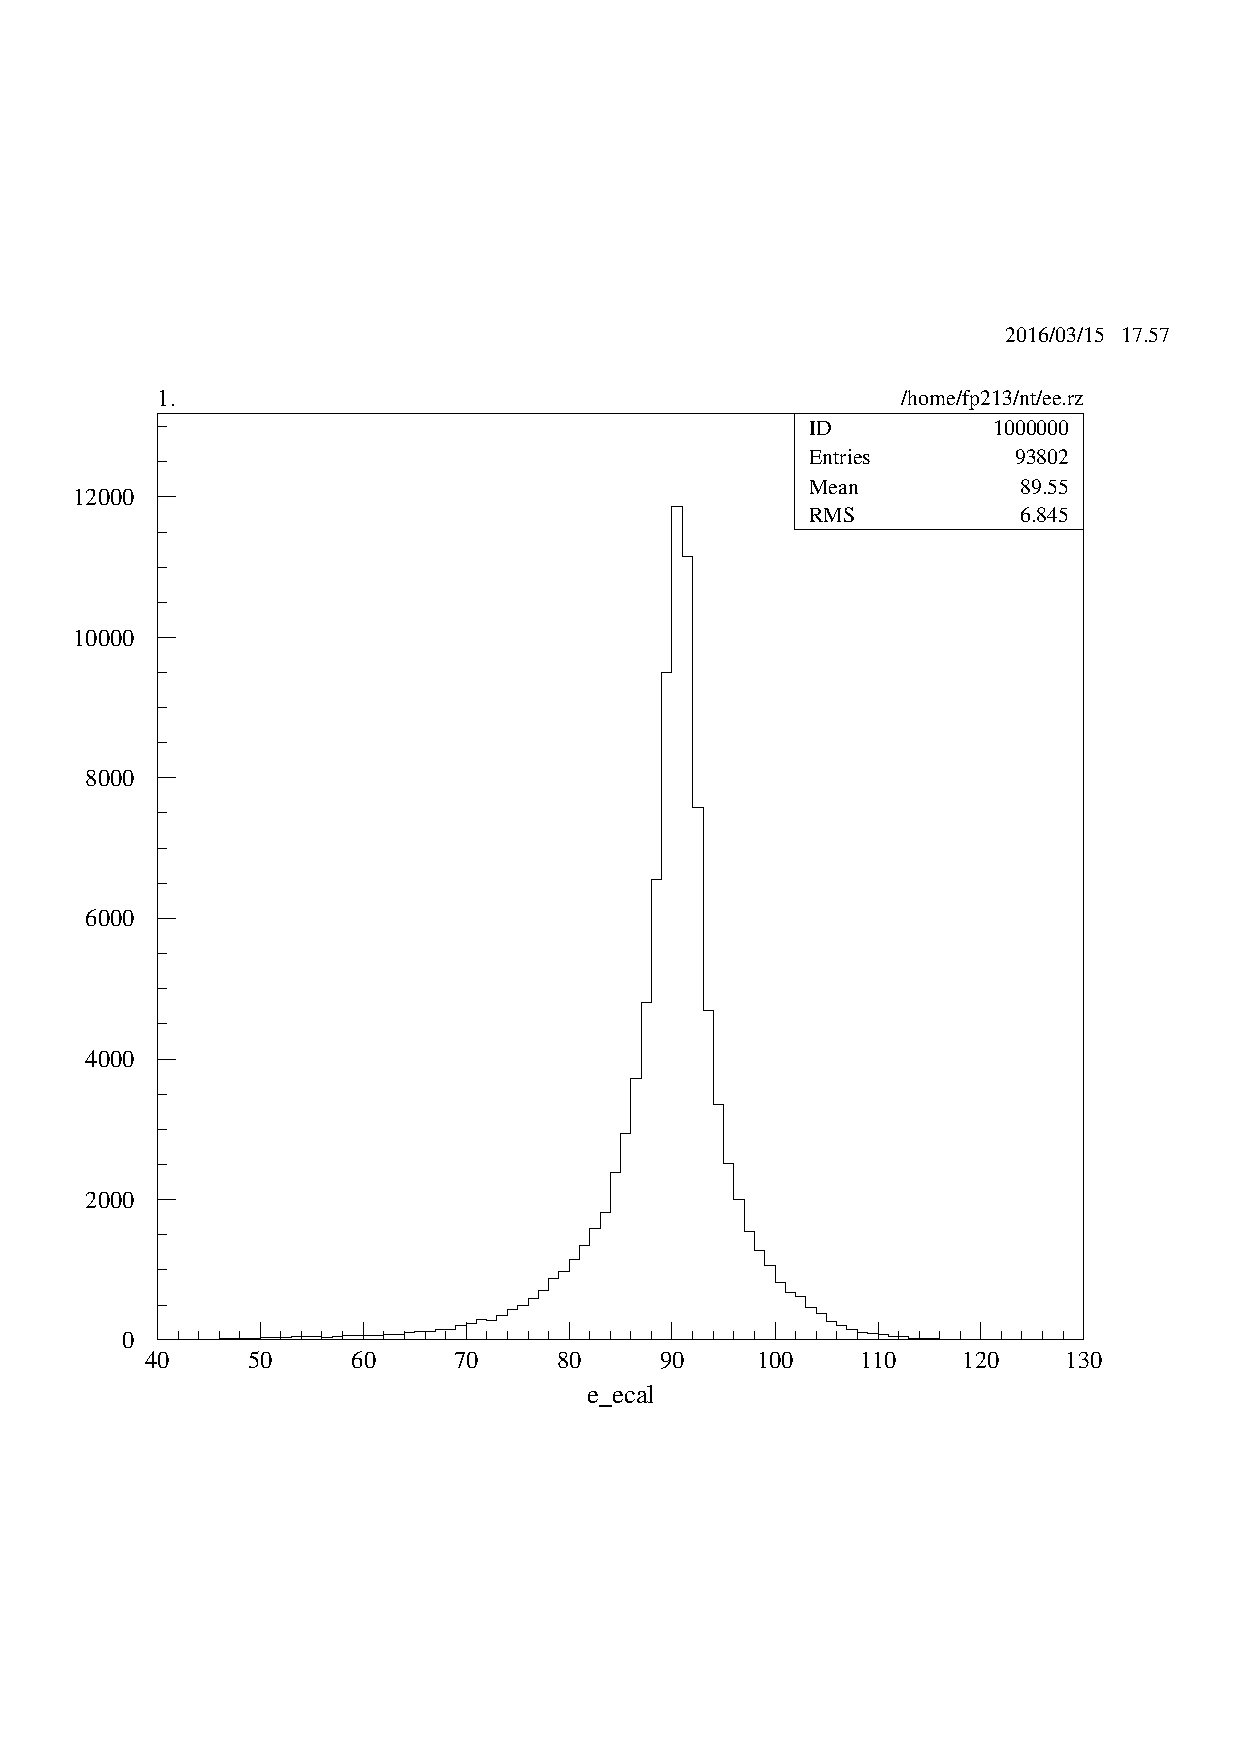
\includegraphics[width=\linewidth]{electrons-e_ecal}
        \caption{%
            Electrons
        }
        \label{fig:paw-e_ecal/electrons}
    \end{subfigure}
    \hfill
    \begin{subfigure}[c]{0.48\linewidth}
        \centering
        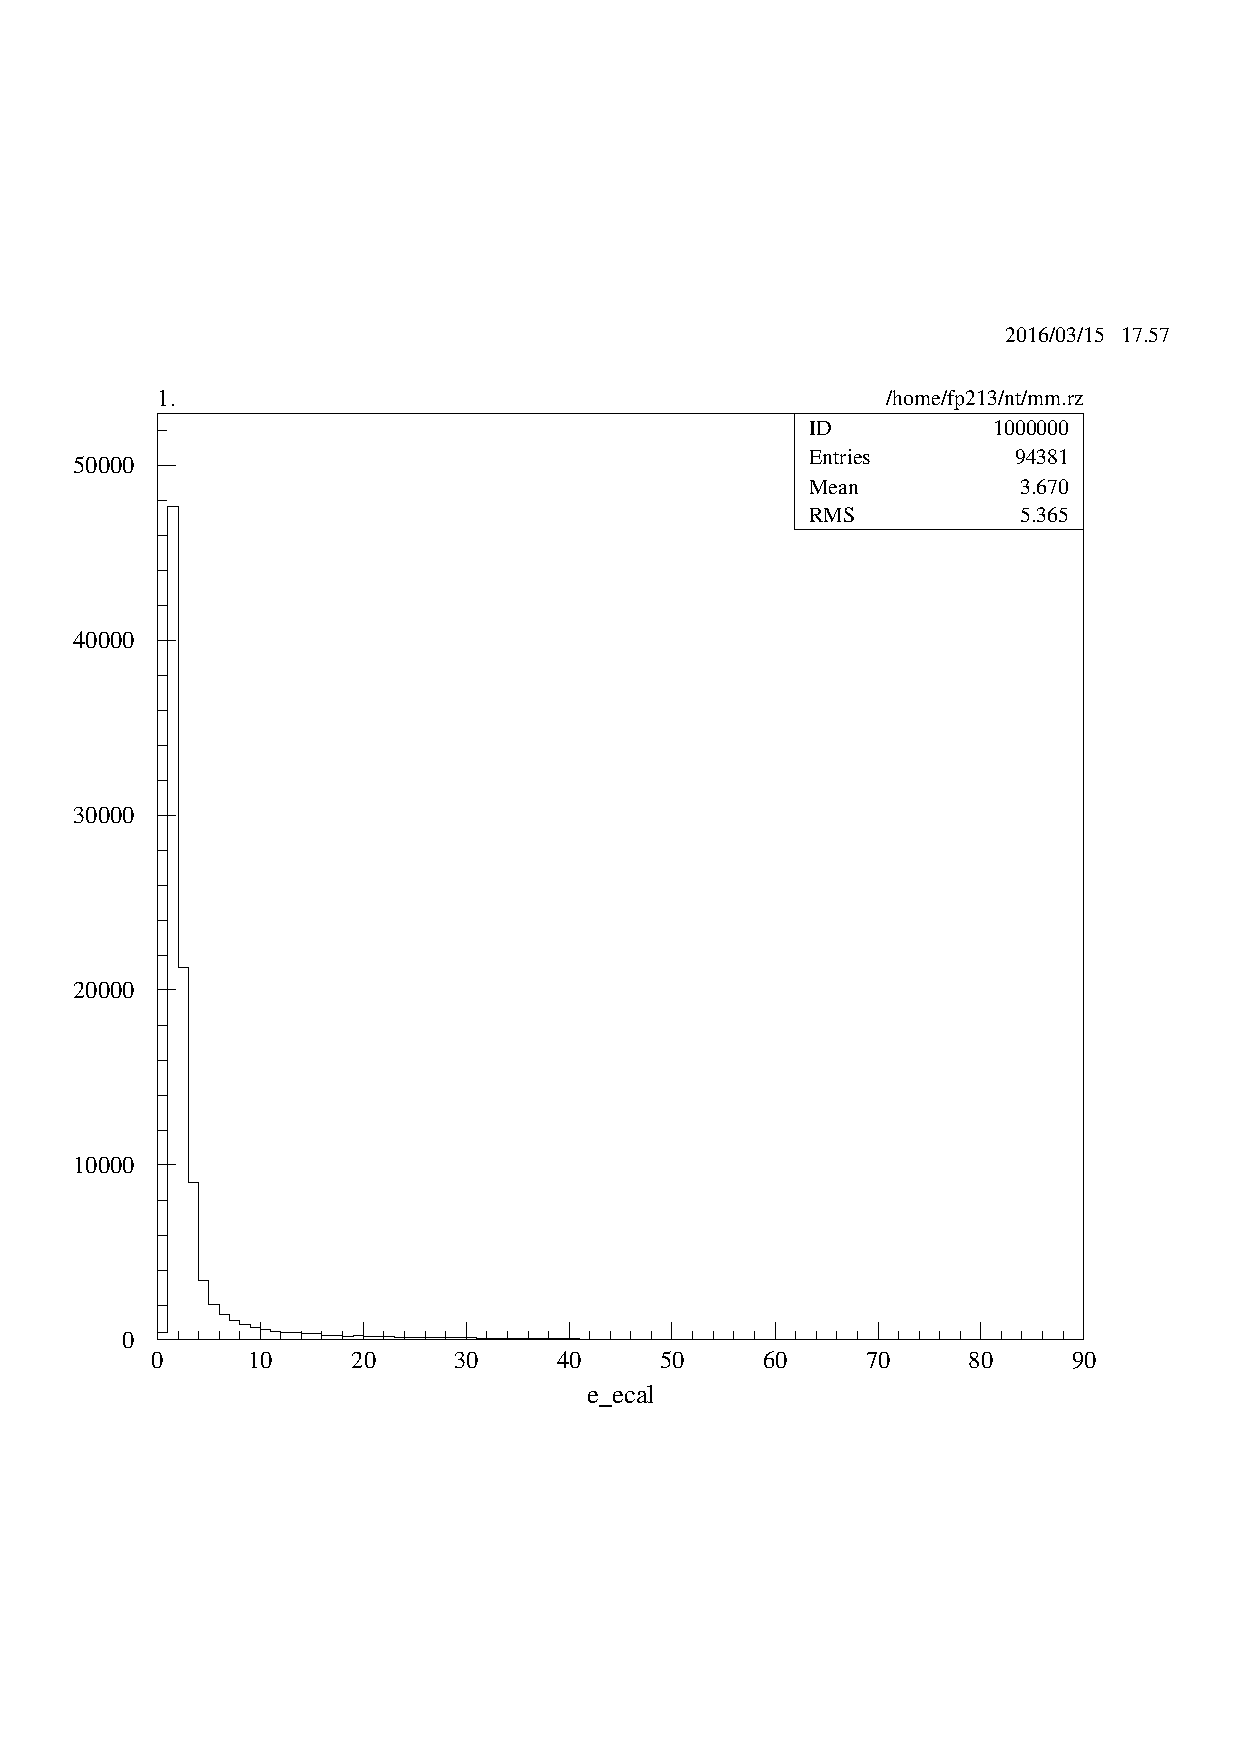
\includegraphics[width=\linewidth]{muons-e_ecal}
        \caption{%
            Muons
        }
        \label{fig:paw-e_ecal/muons}
    \end{subfigure}

    \vspace{2ex}

    \begin{subfigure}[c]{0.48\linewidth}
        \centering
        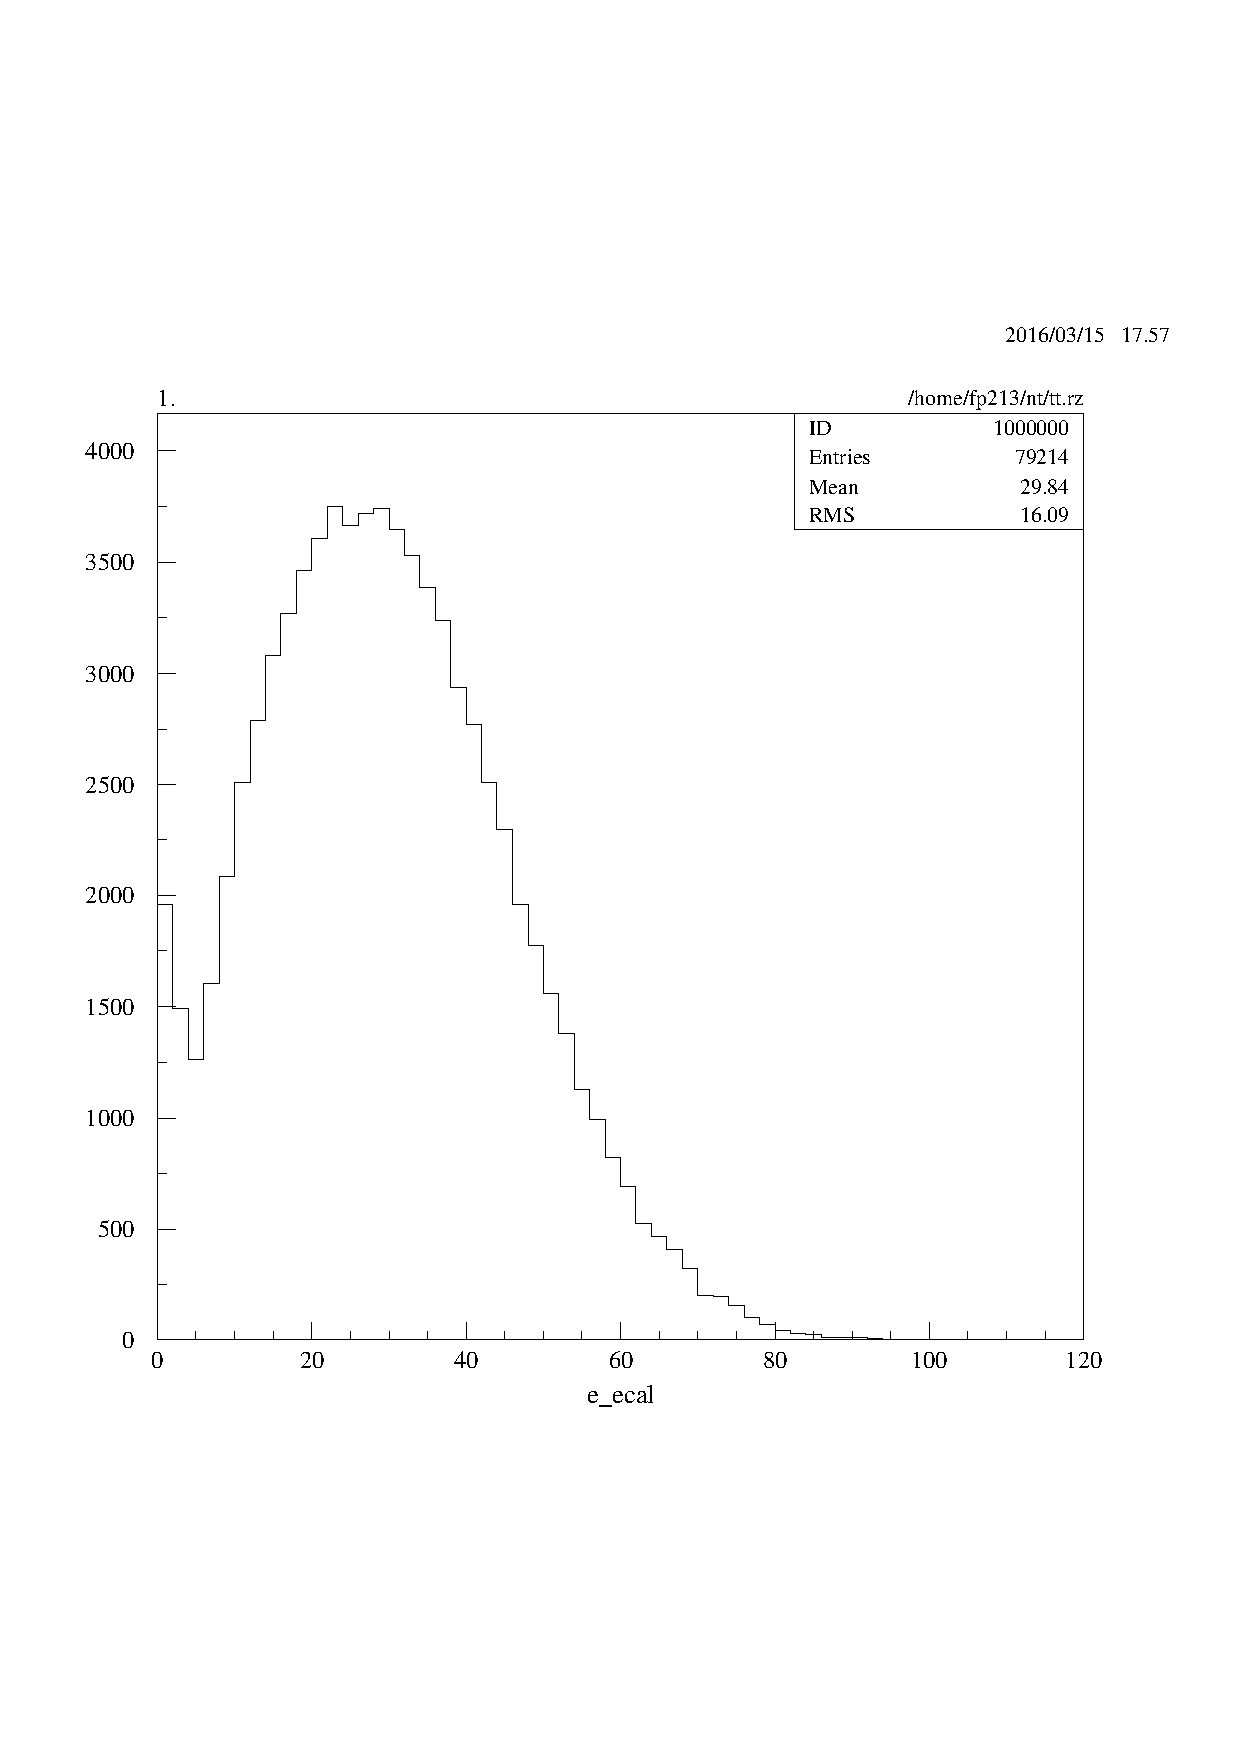
\includegraphics[width=\linewidth]{taus-e_ecal}
        \caption{%
            Tauons
        }
        \label{fig:paw-e_ecal/tauons}
    \end{subfigure}
    \hfill
    \begin{subfigure}[c]{0.48\linewidth}
        \centering
        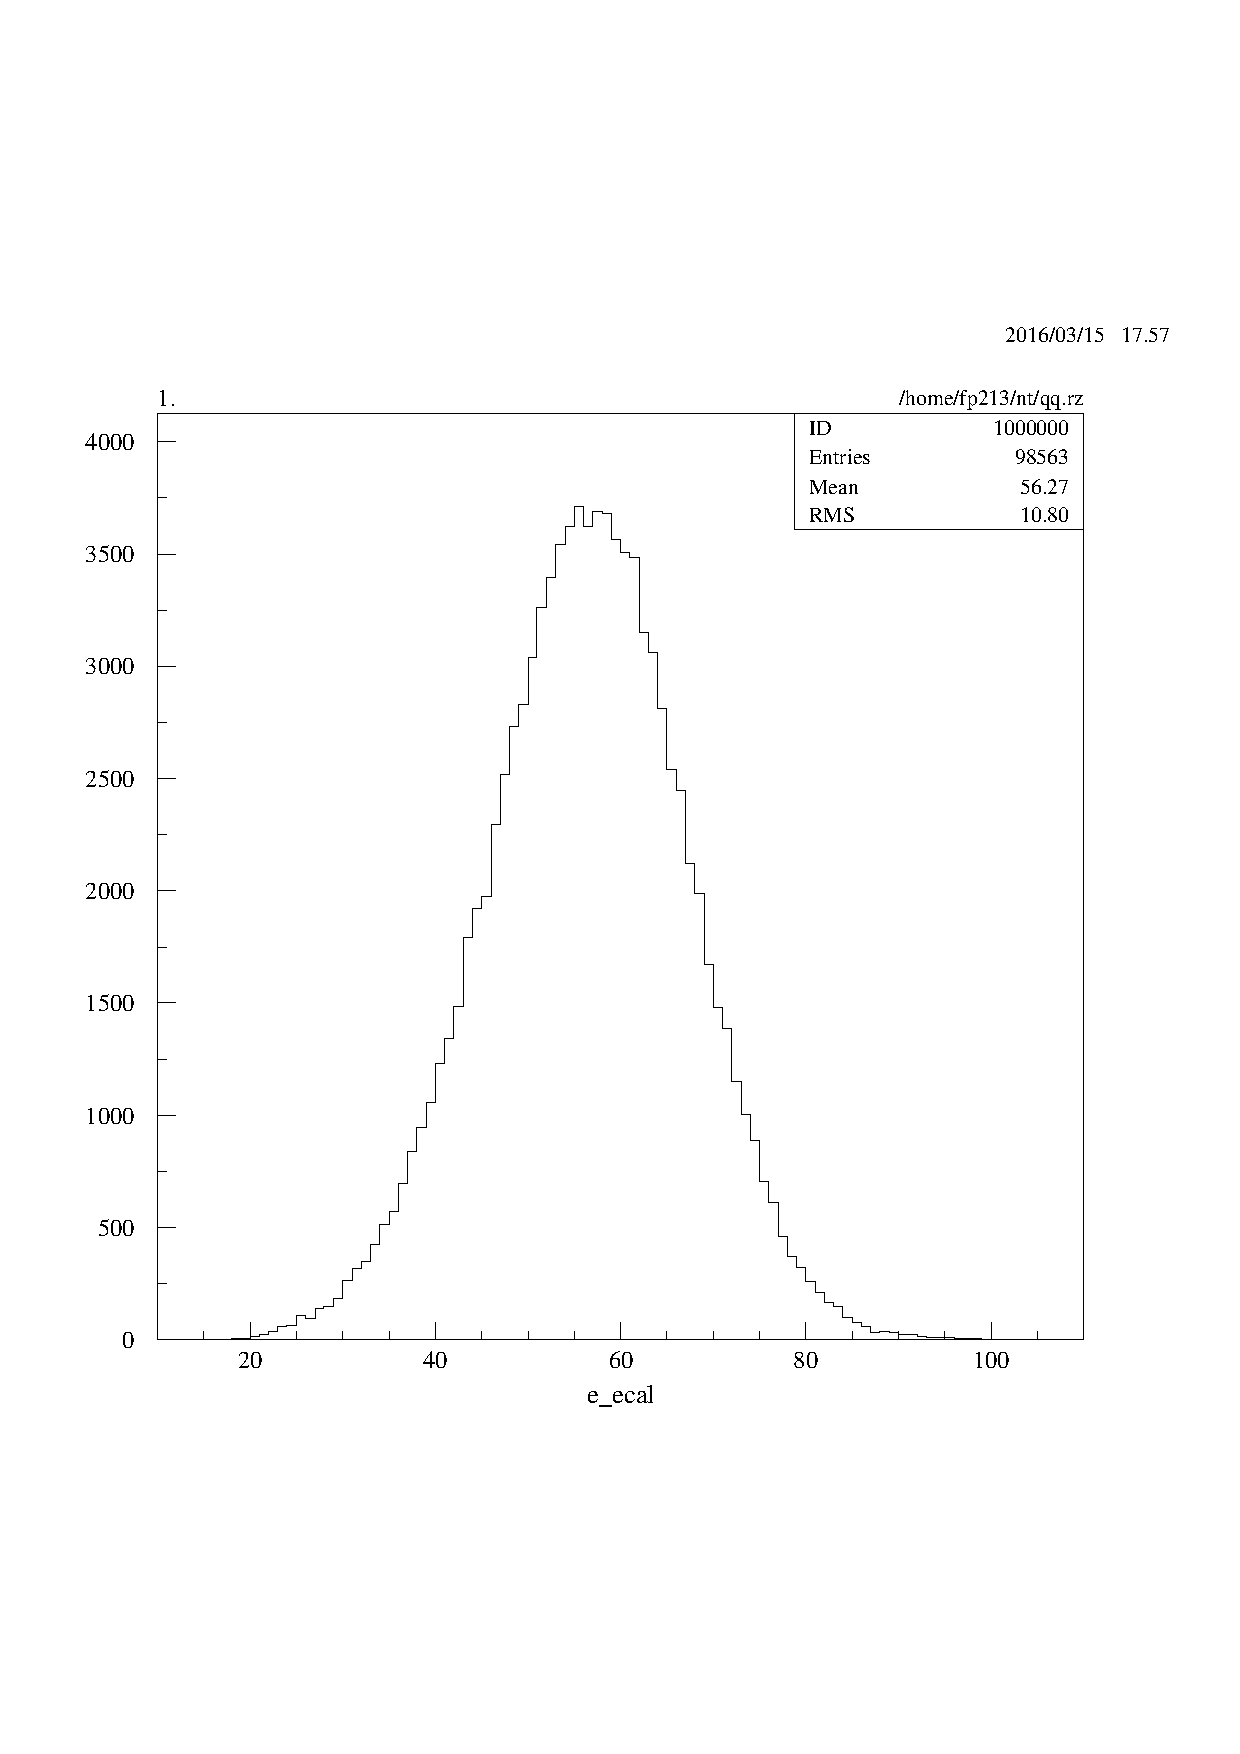
\includegraphics[width=\linewidth]{hadrons-e_ecal}
        \caption{%
            Hadrons
        }
        \label{fig:paw-e_ecal/hadrons}
    \end{subfigure}
    \caption{%
        Energy deposited into the \eecal\ for the four decay types.
        Histograms generated with \textsc{paw} from Monte Carlo datasets.
    }
    \label{fig:paw-e_ecal}
\end{figure}
